In 1915, Albert Einstein published his theory of general relativity, a 
geometric theory of gravitation that sought to expand upon Newtonian 
mechanics and provide a complete description of gravity and its 
relationship with space and time. Einstein theorized that space 
and time were deeply related and existed together as a manifold 
called spacetime. Matter with energy and momentum 
existing in this manifold would create 
curvature in spacetime. Gravitational forces were the result of 
matter following geodesic curves in spacetime. This concept can 
be summarized in the Einstein field equation, which is presented 
as,
\begin{equation}
G_{\mu\nu} = 8\pi T_{\mu\nu}
\label{eq:EFE}
\end{equation}
where $G_{\mu\nu}$ is the Einstein tensor, which describes the 
curvature of spacetime, $T_{\mu\nu}$ is the 
stres-energy tensor, which describes the energy and momentum in 
spacetime, and  $G=c=1$. The Einstein tensor is defined as,
\begin{equation}
G_{\mu\nu} = R_{\mu\nu} - \frac{1}{2}Rg_{\mu\nu}
\end{equation}
where $R_{\mu\nu}$ is the Ricci curvature tensor and $g_{\mu\nu}$ is 
the metric tensor for the manifold.

An interesting result that arises from this formalism is the 
existence of gravitational waves, which are perturbations in 
spacetime caused by certain types of time-varying mass distributions. 
To describe gravitational waves, we consider 
a Minkowski metric with a small perturbation. The Minkowski metric 
is a flat spacetime metric defined as
\begin{equation}
\eta_{\mu\nu} = 
  \begin{pmatrix}
   -1 & 0 & 0 & 0 \\
    0 & 1 & 0 & 0 \\
    0 & 0 & 1 & 0 \\
    0 & 0 & 0 & 1
  \end{pmatrix}
\end{equation}
where $\mu = 0$ corresponds to the time coordinate and $\mu = {1,2,3}$ 
correspond to the spatial coordinates. In examples, we will use the coordinate 
convention $(x^0,x^1,x^2,x^3) = (ct,x,y,z)$. 
The full spacetime metric, $g_{\mu\nu}$, is then constructed as a 
linear perturbation on the Minkowski metric,
\begin{equation}
g_{\mu\nu} = \eta_{\mu\nu} + h_{\mu\nu}
\end{equation}
where $h_{\mu\nu}$ is the metric perturbation and $|h_{\mu\nu}| \ll 1$.
From here, we follow the convention of Saulson \cite{Saulson:1994} to arrive at the general 
form of a gravitational wave.
At this point it is very useful to move into the transverse traceless 
gauge where coordinates on the manifold are defined by the geodesic 
motion of freely-falling test masses. In this gauge, the weak field 
vacuum solution of the Einstein field equation becomes a wave equation: 
\begin{equation}
\square h_{\mu\nu} = 0.
\end{equation}
The solutions to this differential equation will be plane waves of 
the form
\begin{equation}
h_{\mu\nu} = C_{\mu\nu}e^{i(2\pi ft - \vec{k}\cdot\vec{x})}
\end{equation}
where $C_{\mu\nu}$ is the wave amplitude, $f$ is the frequency, 
and $\vec{k}$ is the wave vector which indicates the direction of 
propagation \cite{Carroll}.

For example, consider the case of a gravitational 
wave propogating along the $\hat{z}$-axis.
When the conditions of the transverse traceless gauge are applied, 
the resulting form of $h_{\mu\nu}$ is 
\begin{equation}
h_{\mu\nu} = 
  \begin{pmatrix}
    0 & 0 & 0 & 0 \\
    0 & h_+ & h_x & 0 \\
    0 & h_x & -h_+ & 0 \\
    0 & 0 & 0 & 0
  \end{pmatrix}
\end{equation}
where the diagonal and off-diagonal terms represent two polarizations 
of the resulting gravitational wave, called "h-plus" and "h-cross" 
respectively.
We can see the effects of this perturbation by observing the  
spacetime interval on the manifold. The spacetime interval is defined as 
\begin{equation}
ds^2 = dx^\mu g_{\mu\nu}dx^\nu.
\end{equation}
Substituting in our perturbed metric for $g_{\mu\nu}$, we find that 
the spacetime interval can be broken up into a standard Minkowski line 
element and a perturbation due to $h_{\mu\nu}$.
\begin{equation}
ds^2 = dx^\mu (\eta_{\mu\nu} + h_{\mu\nu})dx^\nu \\
\end{equation}
\begin{equation}
ds^2 = dx^\mu \eta_{\mu\nu} dx^\nu + dx^\mu h_{\mu\nu}dx^\nu
\label{eq:spacetime}
\end{equation}

As an example, we present the case of a plus-polarized gravitational wave 
propagating in the $\hat{z}$ direction and observe the effect of the perturbation 
on the spacetime interval. The perturbation will have the form 
\begin{equation}
h_{\mu\nu} = 
  \begin{pmatrix}
    0 & 0 & 0 & 0 \\
    0 & h_+ & 0 & 0 \\
    0 & 0 & -h_+ & 0 \\
    0 & 0 & 0 & 0
  \end{pmatrix}
\end{equation}
Using the coordinate convention of $(ct,x,y,z)$, the unperturbed
spacetime interval is given as: 
\begin{equation}
ds^2 = -c^2 dt^2 + dx^2 + dy^2 + dz^2.
\end{equation}
Since the perturbation is spatially transverse to the direction of 
propagation, the ct- and z-coordinates will not be modulated by the 
gravitational wave. The x- and y-coordinates will be modulated  
according to equation \ref{eq:spacetime}. The resulting spacetime 
interval is
\begin{equation}
ds^2 = -c^2 dt^2 + (1 + h_+)dx^2 + (1 - h_+)dy^2 + dz^2.
\end{equation}
This shows that a gravitational wave propogating along the $\hat{z}$-axis 
will differentially stretch and squeeze spacetime in the transverse 
axes. The exact form of $h_+$ will depend on the source of the 
gravitational waves. A visualization of this stretching and squeezing 
is shown in Figure \ref{fig:polarizations}\cite{Polarization}. The cross polarization  
stretches and squeezes at a 45 degree angle relative to the plus 
polarization. The strain, $h_+$, imparted by a gravitational wave is 
typically extremely small by the time it reaches Earth, producing 
differential length changes on the order of $10^{-22}$m. 

\begin{figure}[ht!]
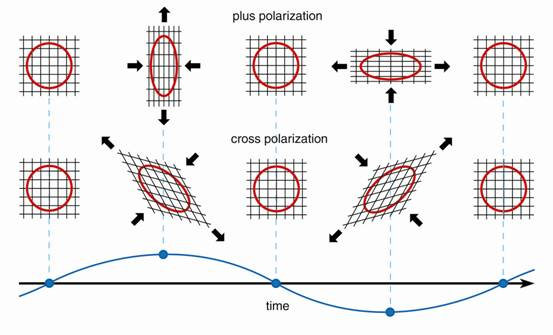
\includegraphics[width=\textwidth]{figures/introduction/polarisations2}
\caption[Plus and cross polarizations]{Plus and cross polarizations %
         of a gravitational wave.}
\label{fig:polarizations}
\end{figure}

The Advanced LIGO interferometers are designed to be sensitive 
to this differential stretching and squeezing by constructing orthogonal 
optical cavities. A gravitational wave passing through an aLIGO interferometer 
will differentially 
modulate the lengths of the optical cavities, creating an interference 
pattern at the output of the instrument that can be searched for 
gravitational wave signals. The layout and gravitational wave readout scheme 
of the interferometers is discussed below.

\section{The Advanced LIGO Interferometers}\label{sec:aligo}

The Advanced LIGO (aLIGO) interferometers are a pair of dual-recycled Michelson interferometers 
that employ 4km long Fabry-Perot cavities in their arms to increase the interaction time with a 
gravitational wave signal. 
Figure \ref{fig:aligo} shows a simplified layout of an aLIGO interferometer. 

\begin{figure}[ht!]
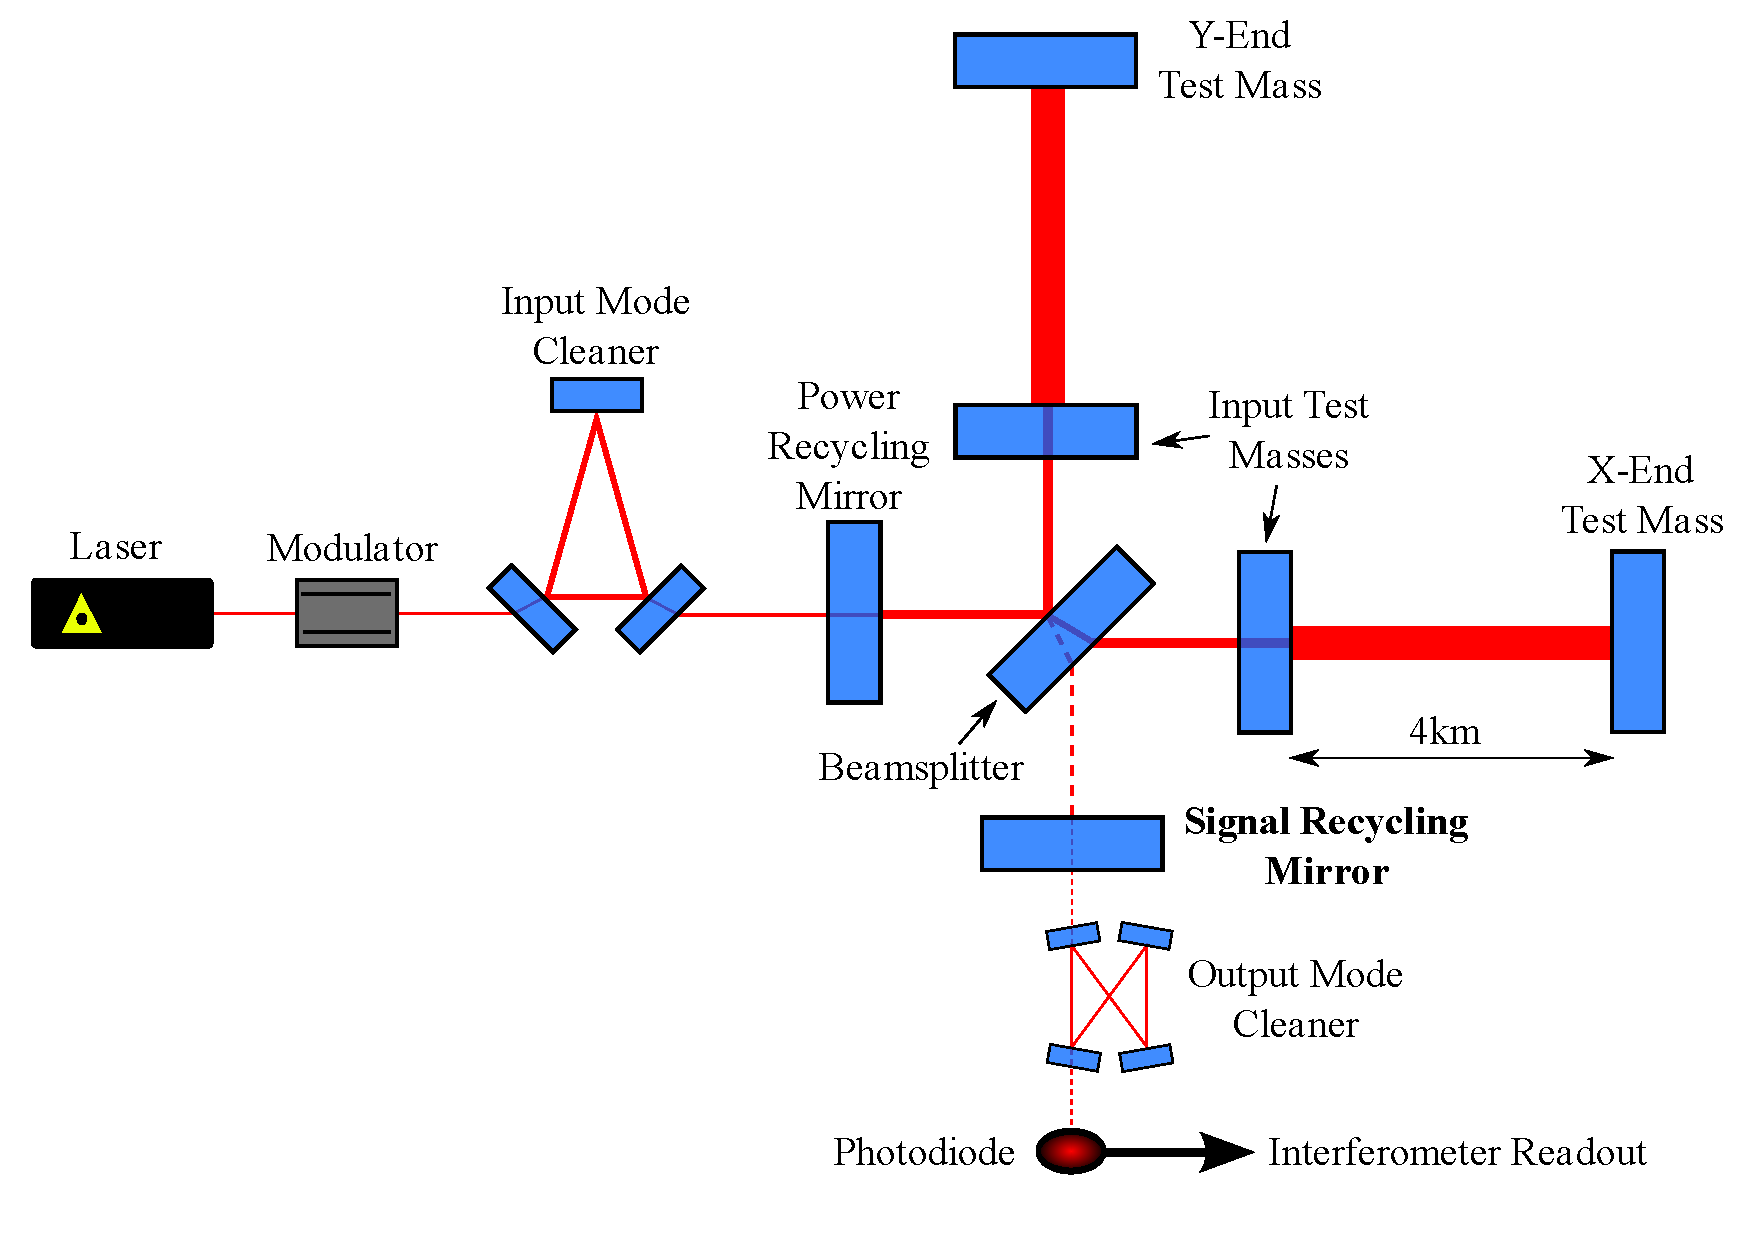
\includegraphics[width=\textwidth]{figures/introduction/ALIGO_layout}
\caption[Layout of Advanced LIGO]{Layout of Advanced LIGO}
\label{fig:aligo}
\end{figure}

At the input to an aLIGO interferometer is a solid-state Nd:YAG laser that provides laser light 
at a wavelength of 1064 nm. Not included in Figure \ref{fig:aligo} are frequency and 
intensity stabilization control loops designed to provide as stable a laser source as 
possible for the experiment. This stabilized laser is called the pre-stabilized laser 
(PSL). The laser light is passed through a series of 
electro-optic modulators (EOM) where radio-frequency (RF) sidebands are generated 
and imparted onto the light. These RF sidebands are used to control auxiliary optical 
degrees of freedom in the interferometer. The beam is then passed through the 
input mode cleaner (IMC), which rejects higher order spatial modes of the beam 
and transmits a circular TEM00 mode to be used in the instrument.

Once the beam has been stabilized in frequency and intensity and the higher order 
optical modes have been stripped away, it is transmitted through the power 
recycling mirror and enters the vertex of the interferometer. In the vertex, 
the beam is split 50/50 by the beamsplitter. Half of the light is directed toward  
the input test mass (ITM) of the X-arm and half of the light is directed  
toward the ITM of the Y-arm. As mentioned previously, the aLIGO arms are not 
single bounce cavities; they are comprised of Fabry-Perot cavities that allow the 
light to circulate in the arm cavities multiple times. The light is stored in 
the arm cavities for $\sim$1ms, trapped between the highly reflective surfaces 
of the ITM and the end test mass (ETM), before it is transmitted back through 
the ITM and into the vertex.

When a gravitational wave passes through an aLIGO inteferometer, the distance
between the ITM and ETM of each arm is modulated, causing the light to have a
longer or shorter travel time as it traverses the arm. Since gravitational
waves expand space in one direction while the orthogonal direction contracts,     
the X- and Y-arms will experience differential changes in length. When light
from the arms is recombined at the beamsplitter, there will be a difference
in phase between the two beams as they have traveled different paths. The 
resulting light from this recombination of phase shifted beams is called the 
antisymmetric part of the output. The part of the beam that is recombined 
in phase is called the symmetric part of the output.

The beams returning from each arm are recombined at the beamsplitter. The 
symmetric part of the beam 
will be sent back toward the power recycling mirror. The power recycling mirror 
forms a resonant cavity with the ITMs, allowing for light at the symmetric 
port of the beamsplitter to be added coherently to incoming light from the PSL and 
increasing the effective power in the vertex. This increase in effective power 
is known as the power recycling gain. 

The antisymmetric part of the beam is sent toward the signal recycling mirror. 
The signal recycling cavity is used to tune the frequency response of the 
interferometer by adjusting the effective finesse of the coupled cavity 
formed by the signal recycling cavity and the arm cavities. 
If the light returning from the arms has accumulated some differential amount of 
phase as it traveled 
along the arms, perhaps from a gravitational wave modulating the length of each 
arm differentially, it will be transmitted through the signal recycling cavity 
and into the output mode cleaner (OMC). The OMC behaves similarly to the IMC, 
stripping away higher order optical modes and isolating the TEM00 mode of the 
beam. The transmitted, mode cleaned signal is then read out using a homodyne 
detection scheme on a DC photodiode. 

\subsection{The aLIGO Noise Curve}

The aLIGO interferometers are among the most precise measuring devices 
that have ever been constructed, sensitive to a differential displacement 
on the order of $10^{-18}$m. When operating at such small length scales, 
the interferometers are susceptible to a number of very subtle noise sources. 
Figure \ref{fig:noise-budget} shows the limiting noise sources for the 
aLIGO interferometers \cite{GW150914-DETECTORS}. Each curve represents 
a known source of noise in the interferometer output. 

\begin{figure}[ht!]
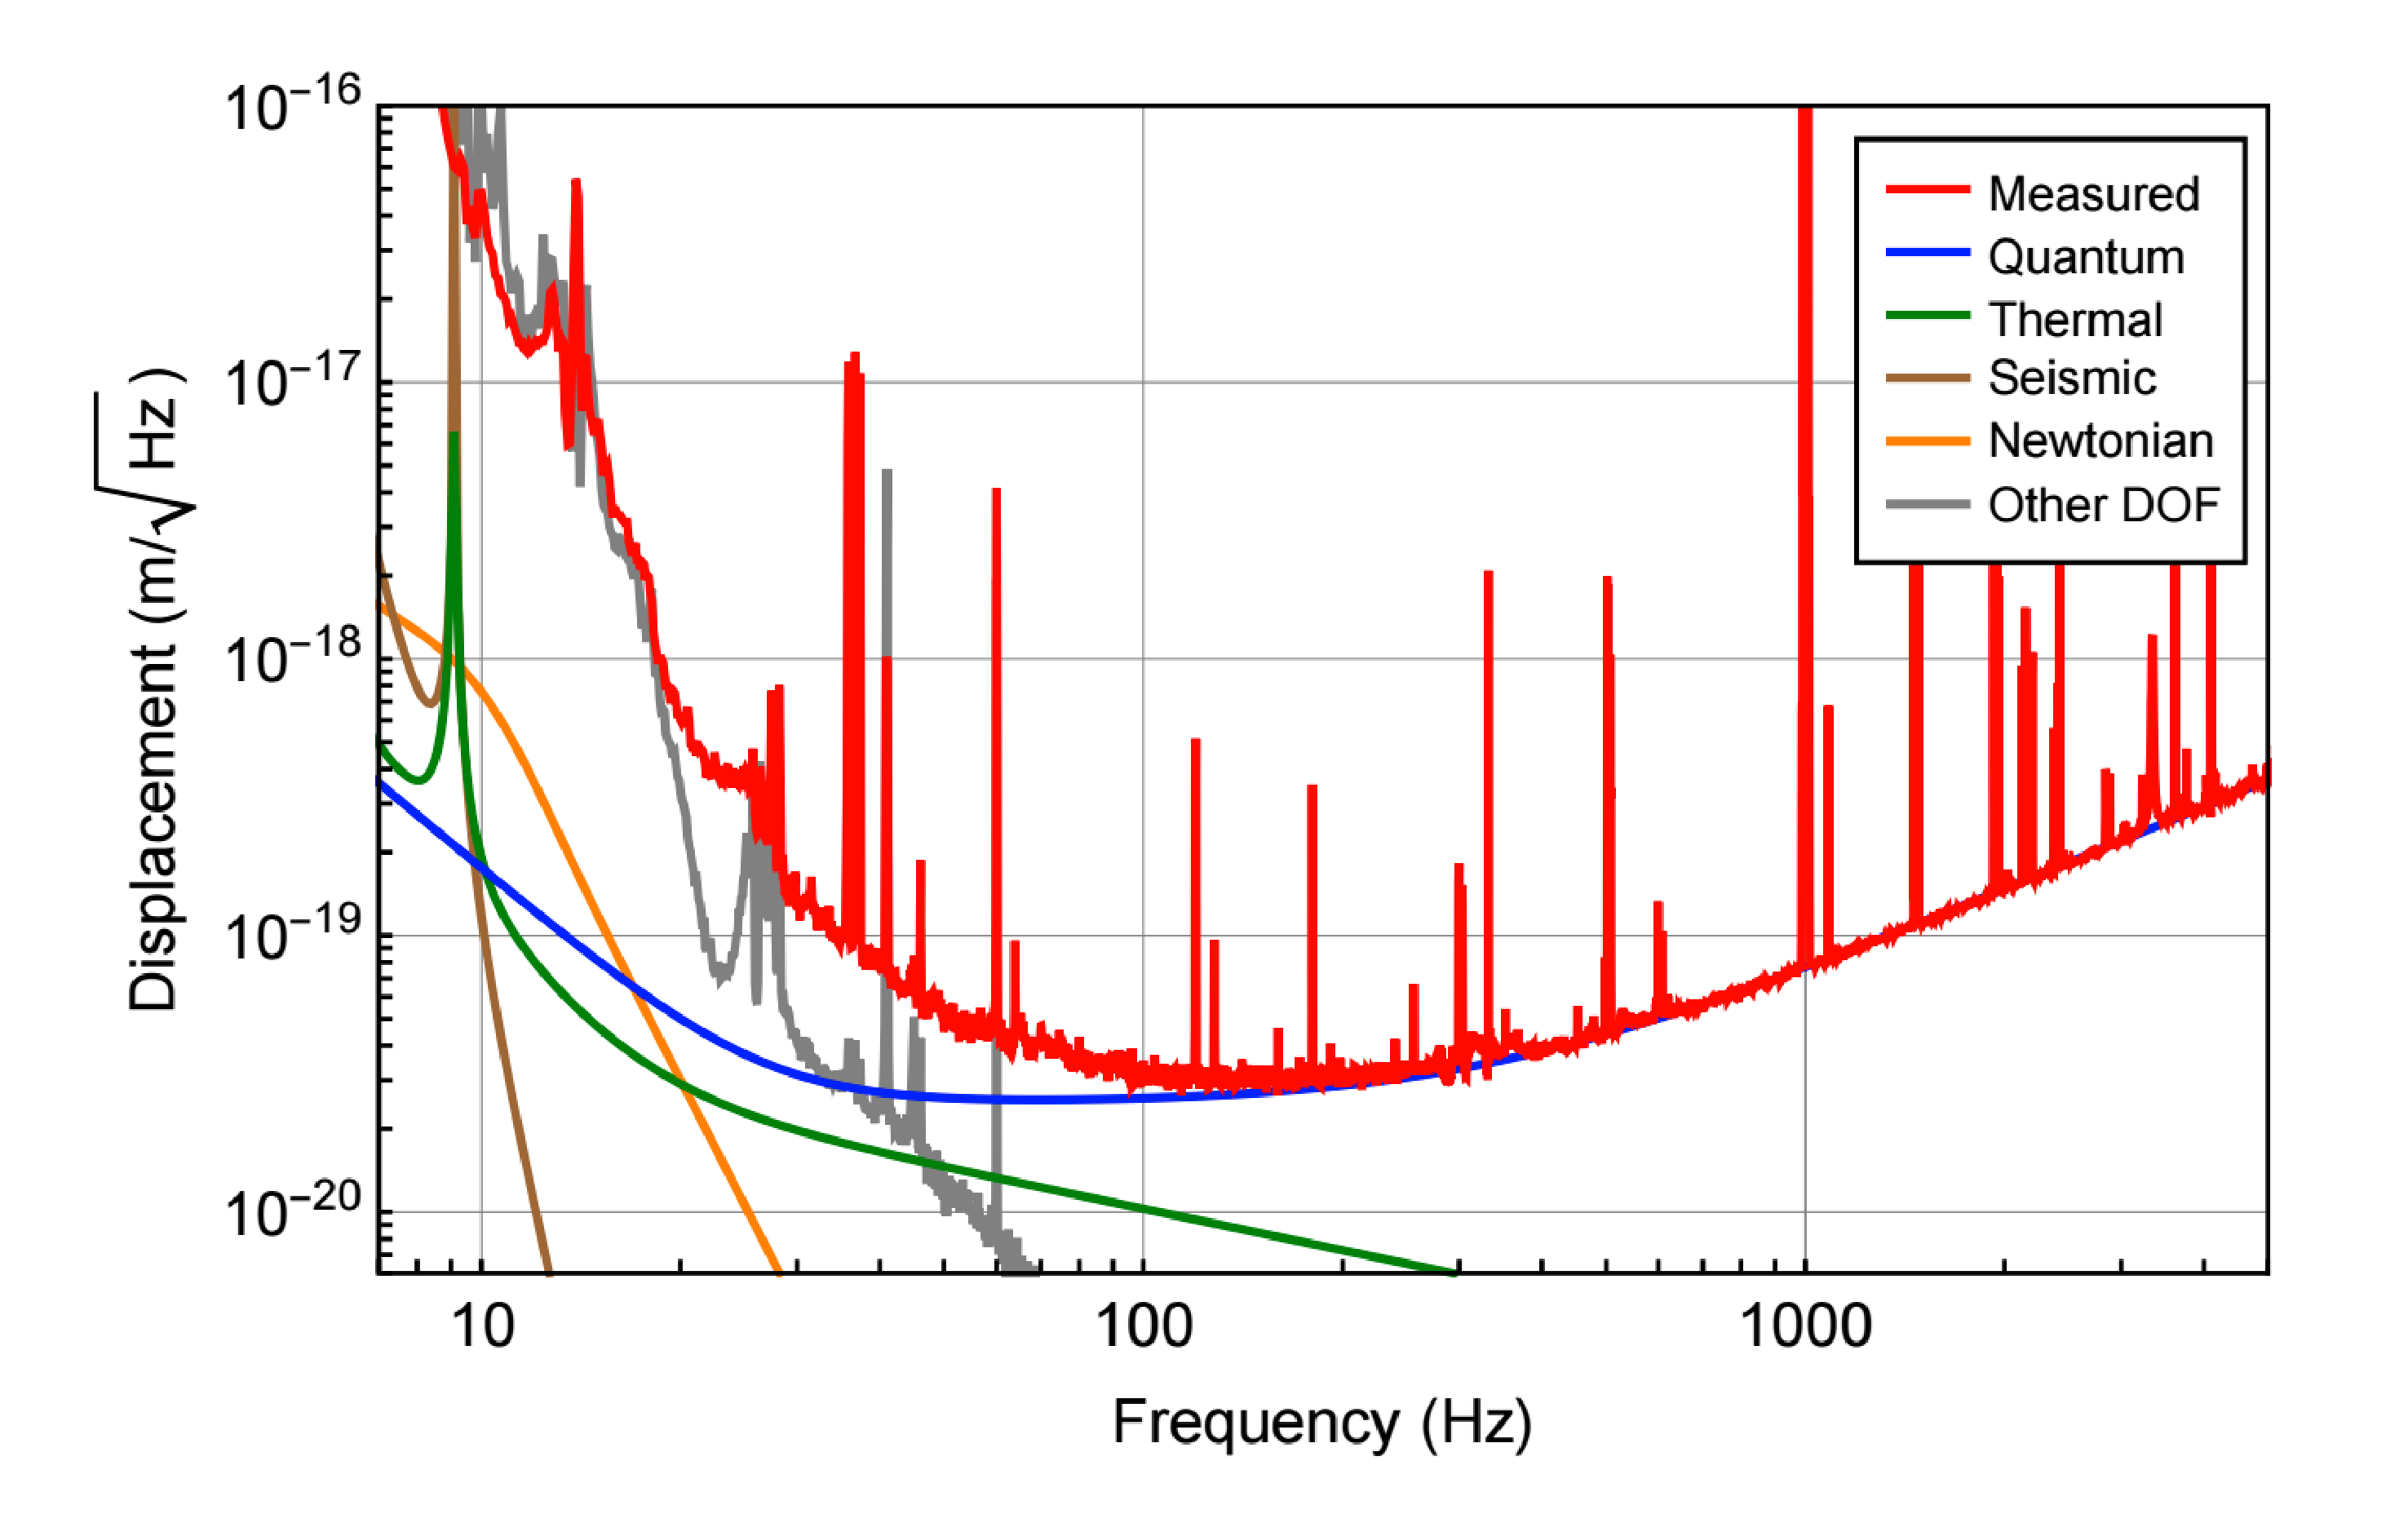
\includegraphics[width=\textwidth]{figures/introduction/noise-budget}
\caption[Advanced LIGO noise budget]{Advanced LIGO noise curve during the first %
         observing run with %
         understood noise sources, reproduced from \cite{GW150914-DETECTORS}. %
         The red curve is the measured instrumental noise at Hanford during the first %
         observing run. The blue curve is quantum noise, which is a combination of %
         photon shot noise at the output photodetector and radiation pressure noise %
         on the test mass optics. The green curve is the modeled thermal noise, which is a %
         combination of thermal noise from the suspensions, optics, and optical %
         coatings. The brown curve is seismic noise coupling into the optics, %
         which is highly attenuated at high frequencies. The orange curve is %
         Newtonian noise, which is driven by perturbations in the density of %
         the ground. The grey curve labeled 'Other DOF' is the sum of the %
         noise coupling from auxiliary optics into the output of the interferometer, %
         mainly driven by optical misalignments.
        }
\label{fig:noise-budget}
\end{figure}

At frequencies below 10 Hz, the limiting noise at design sensitivity 
comes a combination of seismic 
noise and suspension thermal noise. Seismic noise is caused by vibrations coupling 
from the Earth onto the mechanical structures supporting the aLIGO optics. 
Seismic noise is attenuated using 
a multi-tiered active feedback seismic isolation system \cite{SeiReview,HEPI}. At higher 
frequencies, any residual seismic noise is passively attenuated by the 
suspension systems, which use multiple stages of pendula to reduce displacement noise 
from the suspension point to the optics.
Suspension thermal noise is dominated by the mechanical losses of the fused 
silica fibers used to suspend the test masses. 
Since the interferometers are not yet at design sensitivity, the current 
limiting noise below 10 Hz is driven by noise coupling from auxiliary 
degrees of freedom.

From 10 Hz onwards, there are two dominant noise sources: quantum noise 
(the blue curve in Figure \ref{fig:noise-budget}) 
and coating Brownian noise (the green curve in Figure \ref{fig:noise-budget}). 
Quantum noise is the combination of two sources. 
The first is shot noise, which is a photon counting noise when light is measured 
on a photodiode. Shot noise is the dominant noise source above $\sim$300 Hz and 
can be further improved by increasing laser power. 
The second is radiation pressure noise, which is a fluctuating 
force on the test masses based on fluctuations in photon number in the cavity. 
Radiation pressure noise will increase with increasing laser power as 
a higher photon number implies a higher uncertainty in the momentum 
imparted onto the test mass optics.
Coating Brownian noise is due to thermally driven mechanical losses in optical 
coatings. 
Figure \ref{fig:noise-budget} shows that the interferometer noise is 
limited by the combination of thermal noise and quantum noise from 100 Hz 
onward. 
\subsection{DC Readout}

When a gravitational wave modulates the length of an arm cavity, the light 
traveling in that arm experiences a phase modulation. This phase modulation 
can be visualized by picturing the beam in frequency space. In figure 
\ref{fig:omc-freq}, the carrier beam frequency is designated as $f_0$. 
The phase modulation due to 
a gravitational wave signal introduces a frequency sideband at the 
gravitational wave frequency, which is in the 30-2000 Hz range. 
The 
RF sidebands used for auxiliary optical cavity control are offset from the 
carrier frequency by 9, 24, and 45 MHz. 
In a heterodyne detection scheme, the interferometer would operate at the 
'dark fringe', meaning that the output port would not transmit light until 
there was differential arm motion. In this scheme, the RF sidebands would be 
detected on the same photodetector as the gravitational wave sidebands. The 
RF sidebands would be used to demodulate the photodetector signal, leaving 
behind a gravitational wave signal. This is the method that was used in 
initial LIGO.

In Advanced LIGO, a homodyne detection scheme, or 'DC Readout' scheme, is employed 
\cite{DCReadout}. 
In a homodyne detection scheme, the RF sidebands are not used to extract the 
gravitational wave signal. Instead, the carrier beam itself is used. Instead of 
aligning the instrument on the dark fringe, an differential offset is introduced 
to the arm cavities to allow a small amount of light into the output port. 
The RF sidebands, which if not used for demodulation would only contribute 
noise to the output signal, 
are rejected by the output mode cleaner (OMC). 
The gravitational wave sidebands, however, are at a 
low enough frequency offset that they are within the cavity pole of the OMC 
and are allowed to transmit through the cavity.

Since the OMC DC photodiode measures power, it measures the square of the 
incident optical field and witnesses beat frequencies between different 
components of the light. If the RF sidebands have been filtered out by 
the OMC, the only remaining beat note will be that of the carrier beam ($f_0$) 
beating against the gravitational wave sideband ($f_0 + f_{GW}$). This beat note will 
appear as the difference in frequency between the two optical fields, 
leaving behind a signal in the 30-2000 Hz range ($f_{GW}$) and providing a 
natural demodulation inherent to the measurement process. 
The process of recovering the gravitational wave sideband using the 
carrier field as a reference is known as homodyne detection. The 
advantage in this method lies in the fact that the carrier beam 
has been passed through the arm cavities. The cavities act as a low 
pass filter and remove high frequency noise relative to the carrier 
beam frequency. The RF sidebands are quite noisy in comparison and this 
noise is propagated forward when they are used for demodulation. 

\begin{figure}[ht!]
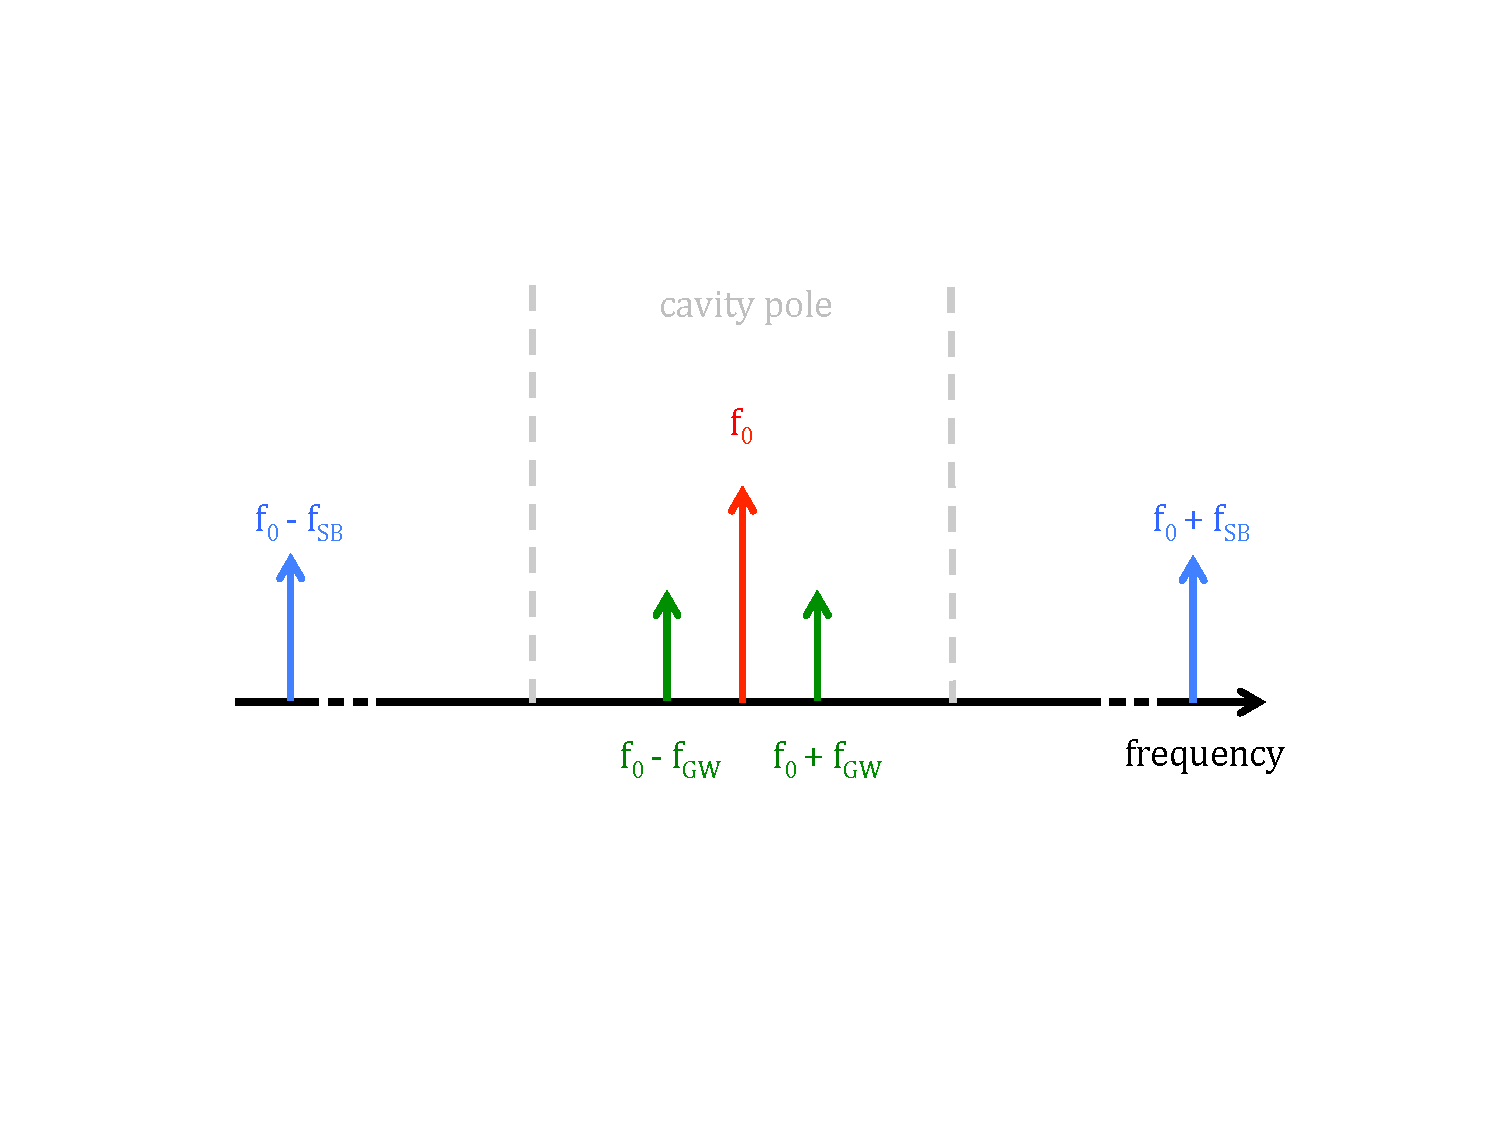
\includegraphics[width=\textwidth]{figures/introduction/omc-freq}
\caption[Sidebands and OMC cavity pole]{Frequency domain visualization of beam %
         at OMC. Grey dotted lines indicate the cavity pole. The gravitational %
         wave sidebands are within the cavity pole and are transmitted through %
         the OMC. The RF sidebands are in the MHz range and are rejected by the %
         OMC.}
\label{fig:omc-freq}
\end{figure}

\section{Sources of Gravitational Waves}

The data at the output of the interferometer must be carefully searched 
for evidence of gravitational wave signals. These signals have highly 
varying characteristics depending on the source of the gravitational 
waves. The gravitational wave strain produced depends on the distribution 
of energy at the source and is given as
\begin{equation}
h_{ij} = \frac{2}{r}\ddot{I}_{ij}
\end{equation}
where $\ddot{I}_{ij}$ is the quadropole tensor describing the 
energy distribution and $c=G=1$. This equation tells us that 
a source distribution requires an accelerating quadropole moment to 
generate gravitational waves. Depending on the dynamics of the source 
system, the resulting gravitational wave signals will vary greatly in 
both duration and morphology.

There are a number of potential sources of gravitational waves that are 
searched for in aLIGO data. Astrophysical searches include both modeled and unmodeled 
searches for both transient and continuous signals. Table \ref{tab:sources} 
gives an example of each of these sources. Each of these categories are 
discussed in the following sections.

\begin{table}[!ht]%
  \begin{tabular}{|c|c|c|}
  \hline
    & Transient  & Continuous  \\
  \hline
  Modeled & Compact binary coalescences & Rotating neutron stars  \\
  \hline
  Unmodeled & Core-collapse supernovae & Stochastic GW background \\
  \hline
  \end{tabular}
  \caption[Table of GW sources]{Table describing sources of %
           gravitational waves.}
  \label{tab:sources}
\end{table}

\subsection{Compact binary coalescences}

Compact binary coalescences (CBC) are a primary search target of the 
Advanced LIGO interferometers. These signals are the result of two 
compact objects, such as neutron stars or black holes, inspiraling 
in a decaying orbit until they merge and coalesce into one final 
compact object. The orbital frequency of such systems increases 
monotonically as the orbit decays, resulting in a gravitational 
wave signal that sweeps upwards in frequency known as a 'chirp'. 
Since the gravitational wave signal from such a system is known, 
this model is incorporated into the search algorithm and the 
search is referred to as a modeled search. CBC waveforms will 
have a duration from $\sim$0.1-60s in the frequency range that
aLIGO is sensitive to and as such they are considered transient 
signals. Searches for CBC 
signals are discussed in Section \ref{sec:cbc-search}.

Of particular interest to aLIGO are binary neutron star systems, 
which are known to exist from astronomical 
observation. The 1993 Nobel Prize in Physics was awared to Hulse and 
Taylor for the indirect detection of gravitational waves from a binary 
neutron star system. The orbital 
period of the Hulse-Taylor binary neutron star system has been measured 
since 1974. The decay of its orbital period matches the 
expected orbital decay based on energy loss due to the emission of 
gravitational waves. 

Beyond binary neutron stars, the search for compact binary coalescences 
is expanded to search for binary black hole (BBH) systems and neutron star-black 
hole (NSBH) systems. The discovery of gravitational waves from binary black holes 
was accomplished in the 
first observing run with the discovery of two binary black hole systems, GW150914 
and GW151226. Further discussion of the results from the first observing run is 
presented in Chapter \ref{ch:o1results}.

\subsection{Burst signals}

An expected population of detectable signals is from unmodeled gravitational 
wave transients, or 'bursts'. These signals can come from core-collapse 
supernovae, cosmic string cusps, and binary black hole mergers 
\cite{Damour:2004kw,GW150914-BURST,lrr-2011-1}. The Advanced LIGO burst 
search is carried out by a number of search pipelines 
\cite{Lynch:2015,BayesWave,Klimenko:2007hd}. 
In a burst search, there are two primary methods for signal identification. 
In a standard burst search, potential signals are identified on a single detector 
basis using an excess power ranking statistic and then checked for coincidence 
between the two interferometers. In a coherent burst search, the data streams 
from both interferometers are combined into one coherent ranking statistic based 
on a maximum likelihood analysis. Each analysis uses their own methods to 
distinguish potential signals from noise.

\subsection{Continuous waves}

Continuous sources of gravitational waves are those that are constantly emitting 
gravitational waves. The primary expected source of continuous gravitational 
waves are rotating neutron stars that have some asymmetry with respect to their 
axis of rotation. If a neutron star has a mountain on it, its rotation will 
produce a time-changing quadropole moment and constantly generate periodic 
gravitational waves. These waves are not expected to be as loud as the 
gravitational waves generated from more violent, transient events. As such, 
the strategy to discover them is different than that of a transient search.

To search for gravitational waves from continuous sources, the data are 
transformed into the frequency domain and integrated for long periods of 
time \cite{CW-all-sky,EinsteinHome}. 
If there is a constant, periodic gravitational wave signal in the data, it 
will manifest as a peak in the frequency spectrum of the data. This peak will 
accumulate signal and grow over the integration period relative to the 
incoherent noise floor. 

\subsection{Stochastic background}

In addition to sources that can be directly detected in the data, there is 
also a search designed to discover a stochastic background of gravitational waves
 \cite{Collaboration:S4Stochastic,GW150914-STOCHASTIC}. 
This stochastic background is the superposition of gravitational wave signals that 
are too weak to be detected directly, such as distant compact binaries and 
supernovae. The stochastic background is a statistical background based on the 
rate and distribution of gravitational wave sources in the universe. To resolve 
the stochastic background, the data from the two interferometers are 
cross-correlated over long periods of time. Since the cross-correlation 
is an integral in the time domain, the effects of quiet, correlated 
gravitational wave signals are accumulated over time until a statistically 
significant signal-to-noise ratio can be quoted \cite{Allen1999Stoch}. 
This is an interesting search from a detector characterization point of view, 
as it requires an understanding of correlated noise sources between the two 
interferometers. 

\section{The Advanced Detector Network}

The Advanced Laser Interferometer Gravitational-Wave Observatory (aLIGO) is 
part of a worldwide effort to detect gravitational waves from astrophysical 
sources. The two aLIGO interferometers, one in Hanford, WA and one in 
Livingston, LA, are part of a growing network of ground-based interferometric 
gravitational wave detectors. Each aLIGO interferometer has 4km long arms 
arranged in an L-shaped configuration. A gravitational wave passing through 
an aLIGO interferometer will cause the arms to expand and contract, 
creating an interferometric signal at the output of the instrument. 
Section \ref{sec:aligo} contains a more detailed description of the aLIGO 
interferometers. 

There are a number of other interferometric gravitational wave detectors 
being built and commissioned for future use in collaboration with aLIGO.
The Advanced VIRGO detector is being built and commissioned in Cascina, Italy. 
When it is fully commissioned, VIRGO will be joining LIGO in observing runs. 
The VIRGO interferometer has 3km arms, which should provide enough 
sensitivity to allow for triangulation of astrophysical sources.

The GEO600 detector, located in Hanover, Germany is an interferometer built in 
collaboration between Germany and the United Kingdom. 
GEO600 is an extremely valuable test bed for interferometric technologies,
including quantum optics and homodyne detection. However, with 600m arms, GEO600 
is unlikely to be sensitive enough to witness expected astrophysical sources.

The KAGRA detector, located underground in the Kamioka mine in Japan, 
is in its commissioning phase. KAGRA has 3 km long arms and, 
unlike other gravitational wave interferometers, employs cryogenics to 
reduce thermal noise in its optics. When complete, KAGRA should be 
sensitive enough to contribute to the worldwide detector network.

Include that cool picture of the advanced detector network.

\section{Searching for Compact Binary Coalescences}\label{sec:cbc-search}

Since the focus of this thesis is the performance of searches for Compact 
Binary Coalescences, a more thorough discussion of how a CBC search 
works is necessary before moving on. 

\subsection{The PyCBC Search Pipeline}

The PyCBC pipeline is designed to search for gravitational wave transients from compact binary
coalescences \cite{Usman:2015kfa}. 
The signals expected to be measured in the aLIGO interferometers are extremely quiet, 
with gravitational wave strains on the order of $10^{-22}$. On these scales, most 
signals will not be able to be extracted from the background noise with simple filtering. 
Figure \ref{fig:quiet-BNS} shows the gravitational wave strain from a 1.4-1.4$M_{\odot}$ 
binary neutron star system at 20 Mpc overlaid on real detector noise from the Livingston 
interferometer. The signal has a peak strain roughly two orders of magnitude lower than 
the peak strain of the detector noise. 
For this reason, the CBC searches employ a matched filter algorithm, which correlates expected CBC
waveforms with detector data and assigns a ranking statistic, the signal-to-noise ratio (SNR),
to every event that it finds. These events are referred to as triggers.
The SNR is defined as 
\begin{equation}
\rho^2(t) = \frac{(s|h_\mathrm{p})^2 + (s|h_\mathrm{c})^2}{(h_\mathrm{p}|h_\mathrm{p})},
\label{eq:snr}
\end{equation}
where $h_\mathrm{p}$ and $h_\mathrm{c}$ are the plus and cross polarizations of the 
modeled gravitational waveform respectively and $s$ is the detector data. The inner product 
is defined as
\begin{equation}
(s|h)(t) = 4\mathrm{Re}\int_{f_\mathrm{low}}^{f_\mathrm{high}} \frac{\tilde{s}(f)\tilde{h}^*(f)}{S_n (f)}e^{2\pi i f t}\, \mathrm{d}f,
\label{eq:inner-product}
\end{equation}
where $\tilde{s}$ is the Fourier transformed detector data, $\tilde{h}$ is the Fourier 
transformed gravitational waveform, and $S_n (f)$ is the power spectral 
density of the detector data averaged over a stretch of 2048 seconds.

The SNR of each trigger is weighted based on a signal consistency test \cite{Allen:2004gu},
resulting in a refined ranking statistic called re-weighted SNR.
Section \ref{sec:chisq} discusses this signal consistency test further.

\begin{figure}[ht!]
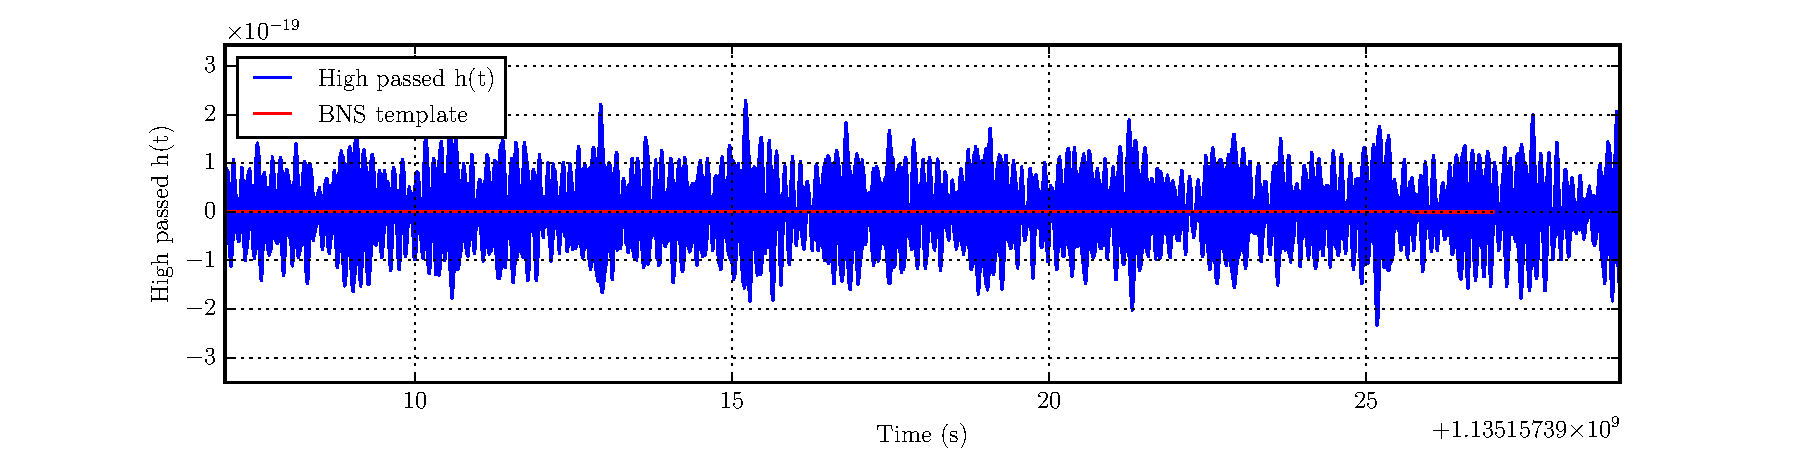
\includegraphics[width=\textwidth]{figures/introduction/quiet_BNS}
\caption[BNS signal in detector noise]{A simulated gravitational wave signal from a %
         binary neutron star system overlaid on real detector noise from L1. %
         The blue curve represents the detector data. The red curve represents %
         the gravitational wave strain expected from a 1.4-1.4$M_{\odot}$ %
         binary neutron star system %
         at 20 Mpc. The peak strain of the binary neturon star waveform is %
         $8\times10^{-22}$. %
         The detector data have been high pass filtered with a corner frequency %
         at 20 Hz and show a peak strain of $2.2\times10^{-19}$. The signal is %
         buried in the detector noise and requires a matched filter algorithm %
         to be recovered. At this time, the inspiral range for a 1.4-1.4$M_{\odot}$ %
         BNS system was 60 Mpc, indicating that the same system originating at 60 Mpc %
         would be recovered with SNR = 8. % 
         }
\label{fig:quiet-BNS}
\end{figure}

To perform this search, the matched filter algorithm needs to know what to search for.
A collection of expected CBC waveforms is generated using
the formalism of general relativity before the analysis.
Each of the expected waveforms is called a template and
the full collection of waveforms is referred to as the template bank. This template bank
is constructed to span the astrophysical parameter space included in the search
\cite{GW150914-CBC}. Each waveform is defined by the mass and spin of each compact
object in the binary system. It is often convenient to combine the effects of each
object's spin into one parameter called effective spin, $\chi_{eff}$,
which is the
mass-weighted spin of the system \cite{Privitera:2013xza}. $\chi_{eff}$ is defined as
\begin{equation}
\chi_{eff} = \frac{\boldsymbol{\chi_{1}}m_{1} + \boldsymbol{\chi_{2}}m_{2}}{m_{1} + m_{2}}
\end{equation}
where $\boldsymbol{\chi_{i}}$ is the dimensionless spin parameter \cite{Kidder:1995zr}
and $m_{i}$ is the
mass for each compact object in the binary system. It is also convenient to combine
the component masses into a new variable, chirp mass, which is used to
parameterize gravitational wave signals in general relativity. Chirp mass is defined
as
\begin{equation}
M_{chirp} = \frac{(m_1m_2)^{3/5}}{(m_1 + m_2)^{1/5}}
\end{equation}
where the $m_{i}$ are once again the component masses of the compact objects in the
binary system.

The search algorithm is run separately at each interferometer and a set of single interferometer
triggers is generated. The two sets of single interferometer triggers are then compared to
search for any events that were recorded within 15ms of each other.
Gravitational waves are predicted by general relativity to travel
at the speed of light. The light travel time between the two interferometers is 10 ms
and 5ms is added to the coincidence window due to uncertainty in signal arrival time
\cite{GW150914-CBC}.
As such, any triggers that are found within 15 ms of each other and
are recovered with the same source parameters are considered to be coincident between the two
interferometers. These coincident triggers represent potential gravitational wave signals
and are referred to as foreground events. Some of these foreground events will be
chance coincidences between noise in each interferometer, which is expected given
the number of events in each data set.

To calculate the statistical significance of foreground events,
a background distribution is generated.
To generate the background, all coincident triggers are removed
from the set of triggers generated for each interferometer, effectively removing all
potential gravitational wave signals from the data set. The remaining triggers are then
a realization of the background noise in each interferometer. These two sets of triggers,
one from each interferometer, are then time shifted by a duration longer than the
light travel time between the interferometers.
Since gravitational waves are predicted to travel at the speed of light,
this time shift ensures that the
two sets of triggers are astrophysically uncorrelated and do not contain any gravitational
wave signals. The coincidence test is then performed again with the time shifted triggers,
resulting in a coincident trigger set which represents background noise alone.
A full distribution of background triggers is generated by performing this timeslide
technique every 0.1 seconds and iterating over all representative, valid data.

The statistical significance of any candidate gravitational wave is
evaluated by calculating the rate of background events from detector noise that are at least as
loud as the candidate event. This statistic is called the false alarm rate (FAR).
Any loud triggers that appear as the result of instrumental
transients will contribute to the tail of the background distribution and
the influence the measured false alarm rate.
The purpose of the data quality effort as a whole is thus two-fold: to ensure that the
search is using nominal, stationary
detector data in the background noise estimation and to suppress the rate of loud events
that will pollute both the background and the foreground distributions.
Two additional stages of data quality that are internal to the PyCBC pipeline, gating and
the $\chi^{2}$ signal consistency test, are discussed below.

\subsection{Gating}\label{sec:gating}

The PyCBC search includes a data conditioning stage that effectively applies preventative data quality
cuts on the input data stream. This is done in a process called gating \cite{Usman:2015kfa}, which uses a
window function to remove times containing large transients from the input data stream. This is done
by applying a smooth windowing function to the problematic section of data,
excising the large transient.
The gating process is tuned by modifying the selection criteria for transients to be removed and
by adjusting the time window to remove around each transient.

For the first analysis block, from September 12 - October 20, 2015, an external transient
identification algorithm called Omicron \cite{Robinet:2015om}
was used to build the list of gating windows. A conservative threshold was set at Omicron SNR $>$ 300
to indicate a transient that should be gated. At each of these times a 1 second time window was constructed,
centered around the time of the transient, that indicated the stretch of data to be removed from the analysis.
This is the gating strategy that was employed in the analysis that included GW150914.
GW150914, which is considered to be a strong gravitational wave signal, was recovered by Omicron with an SNR
of 13 and 9 at Hanford and Livingston respectively, well beneath the gating threshold.

In the analysis containing GW151226, a different method was used to remove data at the
input to the search. Instead of relying on an external process to identify large transients,
an internal test is used to find large excursions in the input data \cite{Usman:2015kfa}.
The time domain input
data are Fourier transformed into the frequency domain and whitened using the
measured power spectral density. The data are then inverse Fourier transformed back into
the time domain and compared to a threshold value set to perform comparably to the
Omicron gating process.
If the whitened data have excursions that exceed this threshold, a gating window is
constructed to remove these data from the input to the search.
Tests were done to ensure that loud signals would not be
removed by the auto-gating process.

\subsection{$\chi^{2}$ signal consistency test}\label{sec:chisq}

A further layer of effective data quality that is internal to the PyCBC pipeline is the application of the
$\chi^{2}$ signal consistency test \cite{Allen:2004gu}. The SNR produced by the matched filter in PyCBC is an
integral in the frequency domain. The $\chi^{2}$ test divides each CBC waveform into
frequency bins of equal power, checking that the SNR is distributed as a function of frequency
as expected from an actual CBC signal.
For a signal divided into $p$ frequency bins, each bin should contain $\frac{1}{p}$ of the power in the 
signal. 
In the $\chi^2$ calculation, the SNR is calculated for each frequency bin and compared to the expected 
amount. The $\chi^2$ statistic is calculated as \cite{Usman:2015kfa}
\begin{equation}
\chi^2 = p\displaystyle\sum_{l=1}^{p}\left[\left(\frac{\rho_\mathrm{p}^2}{p}-\rho_{\mathrm{p},l}^2\right)^2 + \left(\frac{\rho^2_\mathrm{c}}{p}-\rho_{\mathrm{c},l}^2\right)^2 \right] \, ,
\label{eq:chisqr}
\end{equation}
where $\rho^2_\mathrm{p}$ is the SNR of the plus polarization of the waveform, $\rho^2_\mathrm{c}$ 
is the SNR of the cross 
polarization of the waveform, $p$ is the number of frequency bins, and $\rho^2_l$ is the measured SNR 
for the $l^\mathrm{th}$ frequency bin.
The $\chi^2$ statistic is then normalized such that a real signal will be reported with a value of 1. 
This normalized $\chi^2$ is called the reduced $\chi^2$ and is denoted by $\chi^2_r$.

Each trigger that comes out of the matched filter search is down-weighted based on the results of
the $\chi^{2}$ test. This is folded into a new ranking statistic for CBC triggers,
which is called re-weighted SNR and is denoted by $\hat{\rho}$.
The re-weighted SNR is calculated as \cite{Usman:2015kfa} 
\begin{equation}
\hat{\rho} = \left\{\begin{array}{lr}
\rho\left/\left[(1+(\chi^2_r)^3)/2\right]^\frac{1}{6}\right., & \text{if } \chi_r^2 > 1, \\
\rho, & \text{if } \chi_r^2 \le 1,
\label{eq:reweighted}
\end{array}\right.
\end{equation}
where $\rho$ is the measured SNR and $\chi^2_r$ is the reduced $\chi^2$.
It is important to note that if a real signal has a power
distribution that matches the template waveform, it will not be
down-weighted by the $\chi^{2}$ test. The reduced $\chi^2$ will be at a value of 1 
and SNR and the re-weighted SNR will equal.

The ranking statistic for coincident events in the PyCBC search is the network
re-weighted SNR, $\hat{\rho}_{c}$, which is the quadrature sum of the re-weighted
SNR from each interferometer.  
\begin{equation}
\hat{\rho}_{c} = \sqrt{\hat{\rho}^2_L + \hat{\rho}^2_H}
\end{equation}
where $\hat{\rho}_L$ is the re-weighted SNR measured in the Livingston detector 
and $\hat{\rho}_H$ is the re-weighted SNR measured in the Hanford detector.

This test is extremely powerful, as shown in Figure \ref{fig:cbc-newsnr-histograms}, which shows the
distribution of single detector PyCBC triggers generated from September 12 to October 20, 2015.
Figure \ref{subfig:l1-snr-hist} shows the distribution of triggers in SNR. The extensive tail of
triggers with high SNR, which extends beyond SNR 100, is down-weighted in the re-weighted SNR distribution,
leaving behind a tail that extends to $\hat{\rho} \approx$ 11.5 as seen in Figure \ref{subfig:l1-newsnr-hist}.
This re-weighted SNR tail represents the loudest triggers in the CBC search. Investigating this set of
loudest background triggers guides data quality efforts in defining the current limiting noise sources
to the CBC search.

\begin{figure}[!ht]%
\centering
  \subfloat[]{
      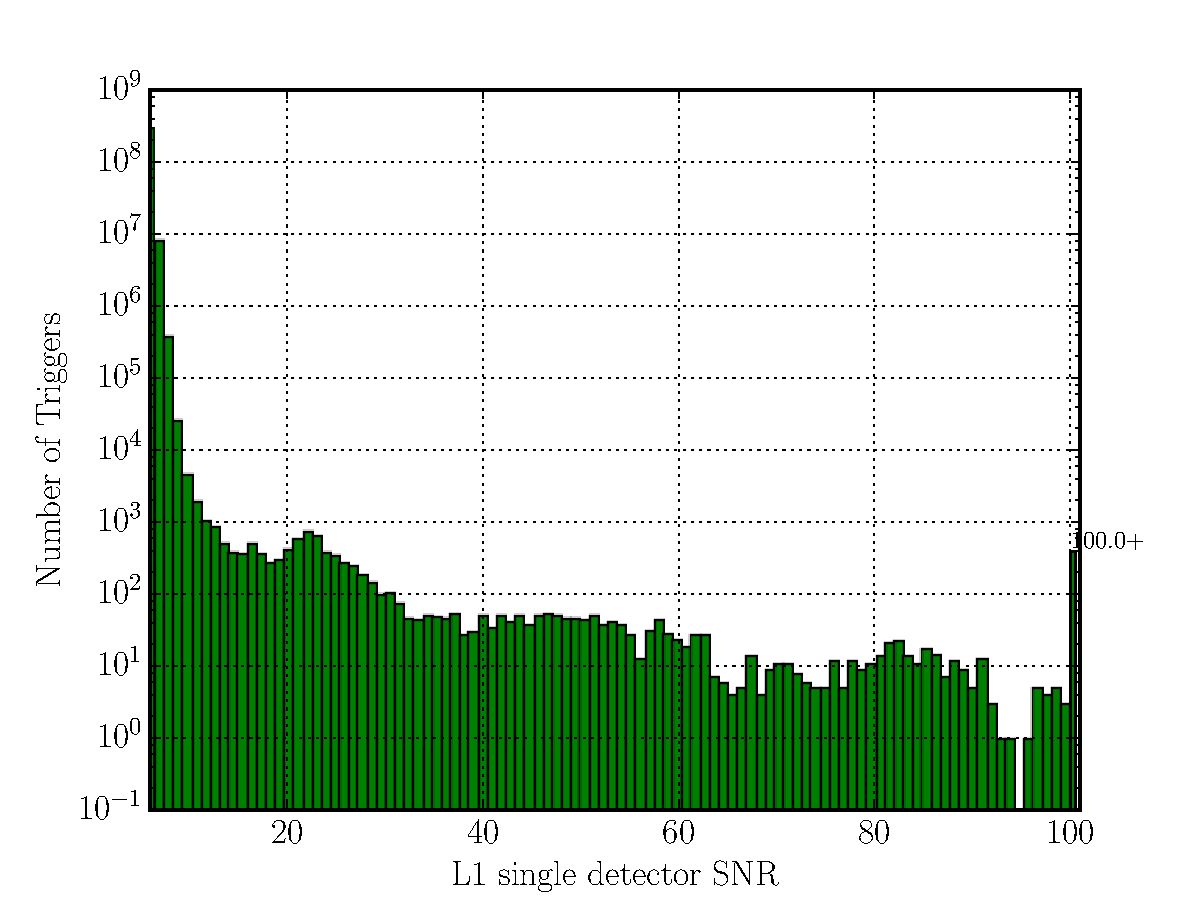
\includegraphics[width=.75\textwidth]{figures/introduction/l1-snr-histogram}
      \label{subfig:l1-snr-hist}
  }

  \subfloat[]{
      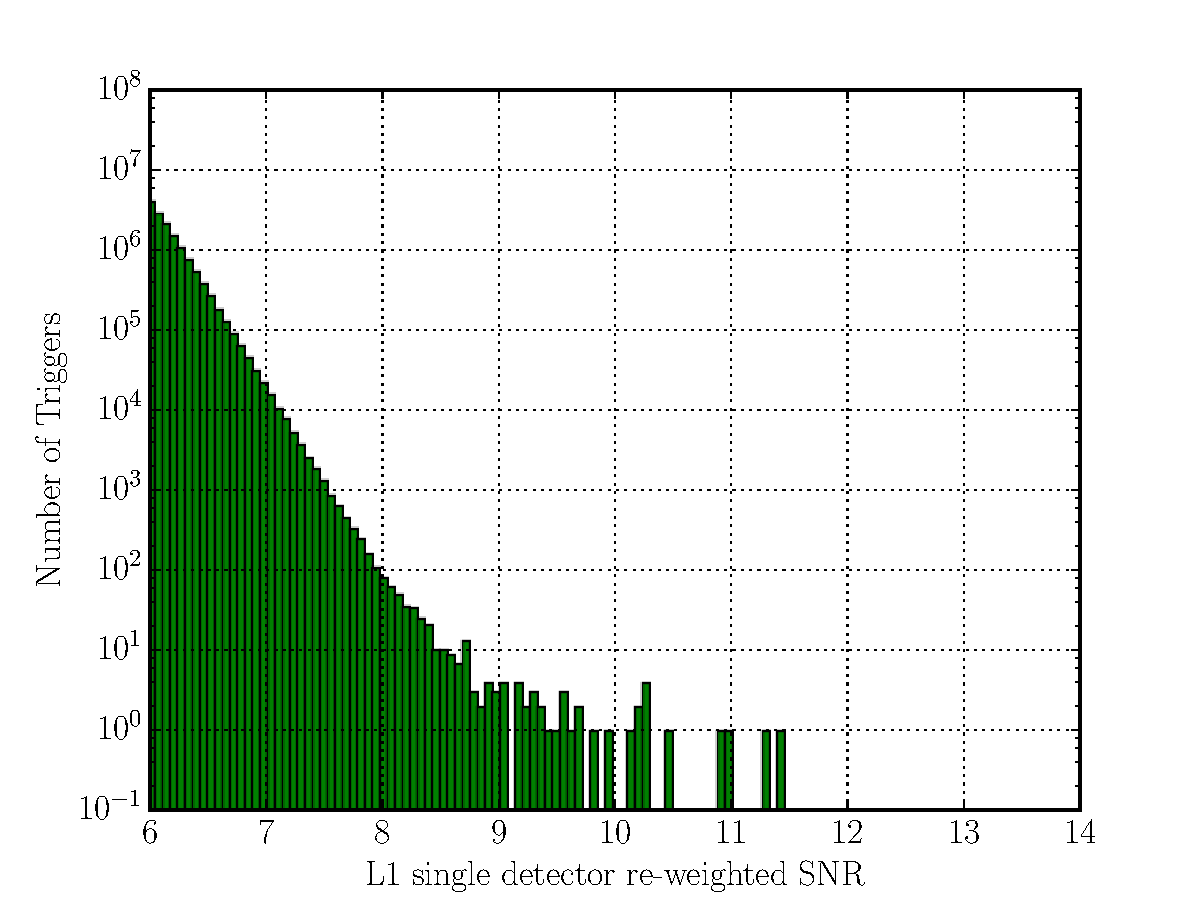
\includegraphics[width=.75\textwidth]{figures/introduction/l1-newsnr-histogram}
      \label{subfig:l1-newsnr-hist}
  }

  \caption[PyCBC SNR and re-weighted SNR histograms]{Histograms of single interferometer PyCBC %
           triggers from the Livingston (L1) interferometer. %
           These triggers were generated from September 12 to October 20, 2015. These histograms %
           contain triggers from the entire template bank, but %
           exclude any triggers found in coincidence between the two interferometers. %
           (\ref{subfig:l1-snr-hist}) A histogram of single interferometer triggers in SNR. %
           The tail of this distribution extends beyond SNR = 100. %
           (\ref{subfig:l1-newsnr-hist}) A histogram of single interferometer triggers in re-weighted SNR. %
           The chi-squared test down-weights the long tail of SNR triggers %
           in the re-weighted SNR distribution.}
  \label{fig:cbc-newsnr-histograms}
\end{figure}

